% Project Overview — Building Energy Prediction
% Compile: pdflatex project_overview.tex

\documentclass[11pt,a4paper]{article}
\usepackage[utf8]{inputenc}
\usepackage[T1]{fontenc}
\usepackage[margin=1in]{geometry}
\usepackage{amsmath}
\usepackage{booktabs}
\usepackage{enumitem}
\usepackage{hyperref}
\usepackage{xcolor}
\usepackage{tikz}
\usetikzlibrary{shapes.geometric, arrows.meta, positioning, fit}

\definecolor{navy}{HTML}{0f172a}
\definecolor{orange}{HTML}{ea580c}
\definecolor{teal}{HTML}{0d9488}

\tikzset{
  process/.style={rectangle, draw=orange!80, fill=orange!8, align=center, font=\scriptsize, inner sep=2pt},
  output/.style={rectangle, draw=teal!70, fill=teal!10, align=center, font=\scriptsize, inner sep=2pt},
  arrow/.style={-{Stealth[length=1.5mm]}, draw=gray!70},
}

\title{\textbf{Metrik AI: Building Energy Prediction \& Operational Support}\\[0.4em]
\large Scalable forecasting, anomaly detection, and ranked audit for commercial portfolios}
\author{DS-GA 1019 Advanced Python for Data Science \\ ASHRAE GEPIII \,|\, 53.6M hourly readings}
\date{}

\begin{document}
\maketitle

%------------------------------------------------------------------------------
\section{Problem Statement}
%------------------------------------------------------------------------------

Building energy management today is plagued by systemic gaps that leave owners and operators flying blind, spending more than necessary, and missing early warning signs of waste or failure.

\subsection{Lack of visibility}
Most portfolios see only monthly or quarterly utility bills. There is no hourly or sub-hourly view of which meters, zones, or buildings are driving cost. Without granular data and predictions, decisions are based on averages and guesswork.

\subsection{Reactive maintenance}
Issues are discovered only after a complaint, a spike on the bill, or equipment failure. Faulty meters, stuck valves, and equipment left on run for weeks or months before anyone notices, multiplying waste and repair cost.

\subsection{No benchmarking}
Owners cannot easily compare buildings or meters against a reasonable baseline. It is unclear which assets are underperforming, which are efficient, and where to prioritize capital or operational spend.

\subsection{Rising energy costs}
Electricity and gas prices are volatile and often rising. Without predictions and anomaly detection, portfolios cannot optimize when to consume, shift load, or invest in efficiency in a data-driven way.

\subsection{ESG and compliance pressure}
Investors, lenders, and tenants increasingly require emissions and energy reporting. Manual or incomplete reporting is risky and time-consuming. There is a need for auditable, prediction-based baselines and clear evidence of improvement.

\subsection{Inability to detect anomalies in real time}
Even when data exists, few systems automatically compare actual consumption to what was expected and flag sustained deviations. Anomalies that could indicate faults, waste, or fraud go undetected until much later.

\begin{quote}
\noindent\textbf{Core problem:} Building owners lack a scalable, data-driven way to predict expected energy use, detect when reality diverges from that expectation, and prioritize where to act first---all at portfolio scale.
\end{quote}

%------------------------------------------------------------------------------
\section{Our Solution}
%------------------------------------------------------------------------------

We build a scalable, ML-powered pipeline that turns raw meter and weather data into three actionable outputs: predicted consumption, anomaly flags, and a ranked audit list.

\begin{itemize}[noitemsep]
  \item \textbf{Forecasting:} We predict expected energy consumption (e.g., next hour) per meter using leakage-safe features (time, lags, rolling stats, building attributes, weather) and a gradient-boosted model (LightGBM), with simple baselines (e.g., same hour yesterday, per-meter mean) for comparison.
  \item \textbf{Anomaly detection:} We compute residuals (actual minus predicted), normalize by historical variability per meter, and flag anomalies using sustained-deviation rules over a time window. This surfaces faulty meters, equipment left on, and unusual consumption patterns.
  \item \textbf{Ranked audit list:} We aggregate severity (e.g., cumulative positive deviation or count of flagged hours) per meter and per building to produce a prioritized list of where to inspect or intervene first.
\end{itemize}

The pipeline is designed for scale: out-of-core chunked ingestion (e.g., 1--2M rows per batch), merge with building metadata and weather, vectorized feature engineering, optional parallelism by site, and profiling-driven optimization (vectorization, then Numba/Cython where needed). We use the \textbf{ASHRAE Great Energy Predictor III (GEPIII)} dataset: \textbf{53.6 million} hourly meter readings across \textbf{1,636} non-residential buildings, 3,053 meters, 19 sites, two full years (2016--2017), with building metadata and site-level weather.

\noindent\textbf{Deliverables:} Reproducible Python pipeline (CLI, config, tests), benchmark table (baseline vs.\ optimized runtime and memory), a short final report, and an optional Streamlit or React viewer so operators can see forecasts, anomalies, and the audit list in one place.

%------------------------------------------------------------------------------
\section{Why This Is a Real-World Problem}
%------------------------------------------------------------------------------

The problem sits at the intersection of commercial real estate, regulation, and grid operations---with real money and carbon at stake.

\subsection{Commercial real estate scale}
Commercial buildings account for a large share of global energy use and emissions. Portfolios often span dozens to hundreds of buildings and thousands of meters. Decisions made at this scale---where to audit, where to retrofit, how to respond to demand programs---require systematic, data-driven tools, not spreadsheets and intuition.

\subsection{Utility costs}
Energy is one of the largest operating expenses for many building types. Small percentage savings across a portfolio translate into substantial dollar savings. Prediction and anomaly detection make it possible to target the highest-impact opportunities first.

\subsection{Sustainability regulations}
Jurisdictions are imposing disclosure rules, emissions caps, and efficiency standards. Building owners need to measure, report, and reduce consumption in a defensible way. Prediction-based baselines and clear anomaly/audit outputs support both compliance and storytelling.

\subsection{Tenant expectations}
Tenants increasingly expect green buildings, clear sustainability metrics, and stable or reduced operating costs. Owners who can demonstrate efficient operation and continuous improvement have a stronger leasing story.

\subsection{Grid and demand response programs}
Utilities and grid operators run demand response (DR) and flexibility programs. Accurate forecasts help buildings participate effectively---knowing when to curtail or shift load---and capture incentives while avoiding penalties.

\subsection{Insurance and maintenance implications}
Undetected faults can lead to equipment failure, water damage, or safety issues. Early anomaly detection supports preventive maintenance and can reduce insurance and repair costs over time.

%------------------------------------------------------------------------------
\section{Who Benefits and How}
%------------------------------------------------------------------------------

We focus on \textbf{building owners} (and their asset and facility teams) as the primary beneficiaries.

\begin{table}[htbp]
\centering
\small
\begin{tabular}{@{}p{2.2cm}p{9.5cm}@{}}
\toprule
\textbf{Benefit} & \textbf{How the owner gains} \\
\midrule
Direct cost savings & Under gross leases, the owner pays utilities. Lower consumption from better control and early fault detection flows directly to the bottom line. \\
Property value & Efficient, well-instrumented buildings with lower operating costs and strong ESG metrics tend to command higher valuations and better financing terms. \\
Tenant retention & Stable or predictable energy costs and a clear sustainability narrative improve tenant satisfaction and reduce churn. \\
Preventive vs.\ emergency maintenance & The ranked audit list directs limited staff to the worst-performing meters or buildings first. Fixing issues early is cheaper and less disruptive than responding to failures. \\
ESG and emissions compliance & Prediction-based baselines and documented savings support reporting and commitments. Owners can show ``expected vs.\ actual'' and demonstrate continuous improvement. \\
Demand response eligibility & Reliable forecasts make it feasible to enroll in DR and flexibility programs, earning revenue or credits while helping the grid. \\
Competitive differentiation & In tight leasing markets, owners who can show lower operating costs, better sustainability, and data-driven operations stand out to tenants and investors. \\
\bottomrule
\end{tabular}
\caption{Who benefits and how (building owners).}
\end{table}

%------------------------------------------------------------------------------
\section{Gap Analysis}
%------------------------------------------------------------------------------

What exists today versus what we are building:

\begin{table}[htbp]
\centering
\small
\begin{tabular}{@{}p{4.2cm}p{7.5cm}@{}}
\toprule
\textbf{Current state} & \textbf{Our approach} \\
\midrule
Enterprise BMS/analytics: often expensive, vendor-locked, not designed for portfolio-wide ML at 50M+ rows. & Open dataset (ASHRAE GEPIII), reproducible pipeline, standard ML stack. Chunked processing for full scale. \\
Reactive dashboards: show history but do not predict or flag anomalies automatically. & We produce predictions, residuals, anomaly flags, and a ranked audit list so the owner knows where to act first. \\
Manual benchmarking: ad hoc Excel or one-off reports; hard to scale. & Automated, leakage-safe feature engineering and a single pipeline re-runnable as new data arrives. \\
No ranked, actionable output: tools may show ``something is wrong'' but not ``inspect these 10 meters first.'' & We explicitly output a ranked audit list (by meter and/or building) for prioritization. \\
Small-scale or single-building focus: many solutions do not address 50M+ rows or out-of-core processing. & Chunked ingestion, site-based parallelism, profiling-driven optimization (vectorization, Numba/Cython) so the pipeline scales. \\
\bottomrule
\end{tabular}
\caption{Gap analysis: current tools vs.\ our pipeline.}
\end{table}

\noindent\textbf{Summary:} Current tools are either too expensive, not scalable, reactive rather than predictive, or do not produce a single, actionable ranked output. We fill that gap with a transparent, reproducible pipeline built on a public dataset and standard Python/ML tooling.

%------------------------------------------------------------------------------
\section{Project Flowchart}
%------------------------------------------------------------------------------

End-to-end technical flow from raw data to benchmarked outputs. The pipeline runs in batches (e.g., 1--2M rows per chunk), merges with metadata and weather, builds leakage-safe features, trains baselines and LightGBM, computes residuals, scores anomalies, aggregates severity, and produces the audit list---with a profiling and optimization loop to improve runtime and memory.

\begin{figure}[htbp]
\centering
\small
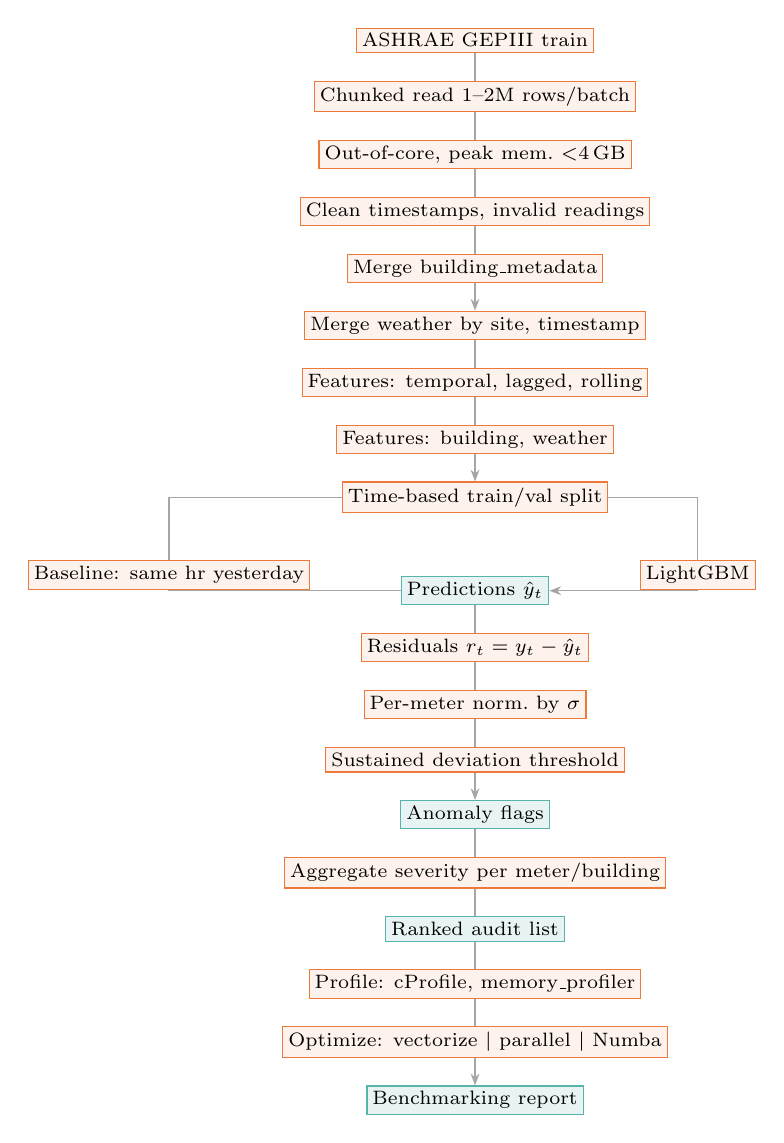
\begin{tikzpicture}[node distance=0.35cm and 0.5cm, every node/.style={font=\scriptsize}]

  \node (a1) [process] {ASHRAE GEPIII train};
  \node (a2) [process, below=of a1] {Chunked read 1--2M rows/batch};
  \node (a3) [process, below=of a2] {Out-of-core, peak mem.\ $<$4\,GB};
  \node (b1) [process, below=of a3] {Clean timestamps, invalid readings};
  \node (b2) [process, below=of b1] {Merge building\_metadata};
  \node (b3) [process, below=of b2] {Merge weather by site, timestamp};
  \node (c1) [process, below=of b3] {Features: temporal, lagged, rolling};
  \node (c2) [process, below=of c1] {Features: building, weather};
  \node (d1) [process, below=of c2] {Time-based train/val split};
  \node (d2) [process, below left=0.6cm and 0.4cm of d1] {Baseline: same hr yesterday};
  \node (d3) [process, below right=0.6cm and 0.4cm of d1] {LightGBM};
  \node (d4) [output, below=0.8cm of d1] {Predictions $\hat{y}_t$};
  \node (e1) [process, below=of d4] {Residuals $r_t = y_t - \hat{y}_t$};
  \node (e2) [process, below=of e1] {Per-meter norm.\ by $\sigma$};
  \node (e3) [process, below=of e2] {Sustained deviation threshold};
  \node (e4) [output, below=of e3] {Anomaly flags};
  \node (f1) [process, below=of e4] {Aggregate severity per meter/building};
  \node (f2) [output, below=of f1] {Ranked audit list};
  \node (g1) [process, below=of f2] {Profile: cProfile, memory\_profiler};
  \node (g2) [process, below=of g1] {Optimize: vectorize $|$ parallel $|$ Numba};
  \node (g3) [output, below=of g2] {Benchmarking report};

  \draw [arrow] (a1) -- (a2) (a2) -- (a3) (a3) -- (b1) (b1) -- (b2) (b2) -- (b3);
  \draw [arrow] (b3) -- (c1) (c1) -- (c2) (c2) -- (d1);
  \draw [arrow] (d1) -| (d2) (d1) -| (d3) (d2) |- (d4) (d3) |- (d4);
  \draw [arrow] (d4) -- (e1) (e1) -- (e2) (e2) -- (e3) (e3) -- (e4);
  \draw [arrow] (e4) -- (f1) (f1) -- (f2) (f2) -- (g1) (g1) -- (g2) (g2) -- (g3);

\end{tikzpicture}
\caption{Raw ASHRAE $\to$ chunked ingestion $\to$ clean \& merge $\to$ leakage-safe features $\to$ baselines + LightGBM $\to$ predictions $\to$ residuals $\to$ anomaly scoring $\to$ ranked audit list $\to$ profiling \& optimization $\to$ benchmarking report.}
\end{figure}

\end{document}
